\documentclass{llncs}
\usepackage{graphicx}

\begin{document}

\title{Un Sistema de Recomendación Híbrido para Mejorar Resultados}
\author{Massiel Paz Otaño \and Marlon Díaz Pérez \and Albaro Suárez Valdes}
\authorrunning{M. Paz, M. Díaz, A. Suárez}
\institute{Facultad de Matemáticas y Ciencias de la Computación, La Habana, Cuba}

\maketitle

\begin{abstract}
En este trabajo se presenta un sistema de recomendación híbrido que combina técnicas de filtrado colaborativo y basado en contenido para mejorar la precisión y relevancia de las recomendaciones en plataformas digitales. El sistema busca superar las limitaciones inherentes a cada enfoque individual, ofreciendo un mecanismo robusto para la personalización de contenidos y productos. A través de un análisis detallado de las interacciones de los usuarios y las características de los productos, se proporciona una metodología que optimiza las recomendaciones adaptándolas a las preferencias de los usuarios. Este enfoque híbrido es evaluado en términos de su capacidad para manejar el problema del "cold start" y para generar recomendaciones de alta calidad en diversos escenarios.
\keywords{Sistemas de recomendación, Filtrado colaborativo, Filtrado basado en contenido, Personalización, Cold start}
\end{abstract}

\section{Introducción}
En la era digital, la sobrecarga de información es un desafío constante para los usuarios que buscan productos o contenido relevante en plataformas en línea. Los sistemas de recomendación han surgido como una solución eficaz para este problema, permitiendo la personalización del contenido y mejorando la experiencia del usuario. Estos sistemas son esenciales en aplicaciones como plataformas de streaming, comercio electrónico, redes sociales, y servicios de noticias, donde juegan un papel crucial en la satisfacción del usuario y el éxito comercial.

Este trabajo tiene como objetivo presentar un sistema de recomendación híbrido que combina técnicas de filtrado colaborativo y basado en contenido para mejorar la precisión y la relevancia de las recomendaciones. La propuesta busca superar las limitaciones inherentes a cada enfoque cuando se emplean de manera aislada, y ofrecer un mecanismo robusto para la personalización de contenidos y productos.

El filtrado colaborativo se basa en la premisa de que los usuarios que han mostrado preferencias similares en el pasado tienden a tener gustos similares en el futuro. Sin embargo, este método enfrenta desafíos en situaciones donde hay escasez de datos, como en el caso de nuevos usuarios o productos, conocido como el problema del "cold start". Por su parte, el filtrado basado en contenido se enfoca en las características intrínsecas de los productos, lo que permite hacer recomendaciones sin depender de la historia de interacciones de otros usuarios, pero puede ser limitado en capturar interacciones complejas.

El sistema híbrido propuesto combina estas dos técnicas para aprovechar sus fortalezas y mitigar sus debilidades, proporcionando recomendaciones más robustas y personalizadas.

\section{Funcionamiento de los Filtros Utilizados}
El sistema de recomendación utiliza dos enfoques principales: filtrado colaborativo y filtrado basado en contenido, cada uno con un proceso específico para evaluar la relevancia de los productos para los usuarios.

\subsection{Filtro Colaborativo}
El \textbf{Filtro Colaborativo} se fundamenta en el análisis de las interacciones pasadas de los usuarios con productos, bajo el supuesto de que usuarios con intereses similares en el pasado compartirán preferencias en el futuro. Los pasos clave del filtro colaborativo incluyen:

\begin{enumerate}
    \item \textbf{Recopilación de Interacciones}: Se recopilan datos de las interacciones de los usuarios, como calificaciones, compras o visualizaciones.
    \item \textbf{Cálculo de Similitudes}: Se calcula la similitud entre usuarios utilizando métricas como la correlación de Pearson o el coseno de similitud.
    \item \textbf{Generación de Recomendaciones}: Se identifican productos que usuarios similares han preferido, pero que el usuario actual aún no ha explorado.
\end{enumerate}

Este método es eficaz en entornos con grandes volúmenes de datos, permitiendo capturar patrones de comportamiento emergentes. No obstante, enfrenta limitaciones en escenarios de escasez de datos, especialmente con nuevos usuarios o productos.

\subsection{Filtro Basado en Contenido}
El \textbf{Filtro Basado en Contenido} se enfoca en los atributos de los productos, recomendando artículos similares a los que un usuario ha interactuado positivamente en el pasado. Los pasos clave incluyen:

\begin{enumerate}
    \item \textbf{Análisis de Características}: Se analizan las características de los productos, creando un perfil detallado.
    \item \textbf{Perfil del Usuario}: Se construye un perfil del usuario basado en sus interacciones previas.
    \item \textbf{Generación de Recomendaciones}: Se recomiendan productos cuyas características coinciden con las preferencias del usuario.
\end{enumerate}

Este enfoque es particularmente útil cuando hay datos limitados sobre las interacciones de los usuarios, y puede capturar las preferencias individuales basadas en atributos específicos del producto.

\section{Ventajas del Enfoque Híbrido}
El sistema híbrido propuesto ofrece varias ventajas en comparación con los enfoques de filtrado colaborativo y basado en contenido por separado:

\begin{itemize}
    \item \textbf{Mejora en la Precisión de las Recomendaciones}: Al combinar ambos enfoques, el sistema puede proporcionar recomendaciones más precisas al aprovechar la información de las interacciones y las características del producto.
    \item \textbf{Mitigación del Problema del Cold Start}: El enfoque híbrido puede manejar mejor el problema del "cold start" al utilizar características del producto para hacer recomendaciones incluso cuando hay pocos datos de interacción.
    \item \textbf{Personalización Más Efectiva}: La combinación de filtrado colaborativo y basado en contenido permite una personalización más efectiva al integrar las preferencias del usuario y las características del producto.
    \item \textbf{Flexibilidad en Diversos Escenarios}: El enfoque híbrido puede adaptarse a diversos escenarios y tipos de datos, proporcionando recomendaciones relevantes en una variedad de contextos.
\end{itemize}

\section{Estructura del Proyecto}
El sistema está organizado en módulos clave, cada uno responsable de un aspecto específico del proceso de recomendación.

\subsection{Filters}
Este módulo implementa las estrategias de recomendación. Se incluyen los siguientes filtros:

\begin{itemize}
    \item \textbf{CollaborativeFilter}: Basado en la similitud de interacciones entre usuarios.
    \item \textbf{ContentBasedFilter}: Basado en la similitud de atributos entre productos.
\end{itemize}

\subsection{Data Access}
Módulo responsable de la gestión y recuperación de datos. Incluye los siguientes repositorios:

\begin{itemize}
    \item \textbf{ProductRepository}: Gestión de datos de productos.
    \item \textbf{CustomerRepository}: Gestión de datos de clientes.
    \item \textbf{InteractionRepository}: Gestión de interacciones usuario-producto.
\end{itemize}

\subsection{Models}
Define los modelos de datos utilizados en el sistema. Incluye:

\begin{itemize}
    \item \textbf{Context}: Información para aplicar filtros, como el ID del usuario y productos relevantes.
    \item \textbf{FilterResultModel}: Representa los resultados de aplicar un filtro.
    \item \textbf{RecommendationModel}: Representa una recomendación individual.
\end{itemize}

\subsection{Services}
Proporciona servicios adicionales que soportan la funcionalidad del sistema, como:

\begin{itemize}
    \item \textbf{Logger}: Registro y seguimiento de actividades del sistema.
\end{itemize}

\section{Implementación y Uso}

\subsection{Configuración}
Para implementar el sistema, siga estos pasos:

\begin{enumerate}
    \item \textbf{Instalación}: Clona el repositorio e instala las dependencias utilizando \texttt{pip}:
    \begin{verbatim}
    pip install -r requirements.txt
    \end{verbatim}
    
    \item \textbf{Infraestructura}: Inicia la base de datos con Docker:
    \begin{verbatim}
    docker-compose up
    \end{verbatim}
    
    \item \textbf{Ejecución}: Inicia la aplicación para generar recomendaciones utilizando las interfaces proporcionadas.
\end{enumerate}

\subsection{Ejemplos de Uso}
Algunos ejemplos incluyen:

\begin{itemize}
    \item \textbf{Aplicar Filtros}: Utiliza el módulo de filtros para generar recomendaciones basadas en usuarios similares.
    \item \textbf{Registro de Actividades}: Utiliza \texttt{Logger} para registrar actividades durante el proceso de recomendación.
\end{itemize}

\section{Conclusión}
El sistema de recomendación híbrido desarrollado en este proyecto demuestra cómo la combinación de filtrado colaborativo y basado en contenido puede mejorar la precisión y relevancia de las recomendaciones. Este enfoque híbrido permite superar limitaciones comunes en los sistemas tradicionales, ofreciendo recomendaciones más personalizadas y efectivas. Además, el sistema muestra mejoras significativas en el manejo del problema del "cold start" y ofrece una solución más robusta para la personalización en diversos contextos.

\section{Imágenes}
A continuación, se incluye una imagen que ilustra el flujo de trabajo del sistema de recomendación híbrido:

\begin{figure}[ht]
\centering
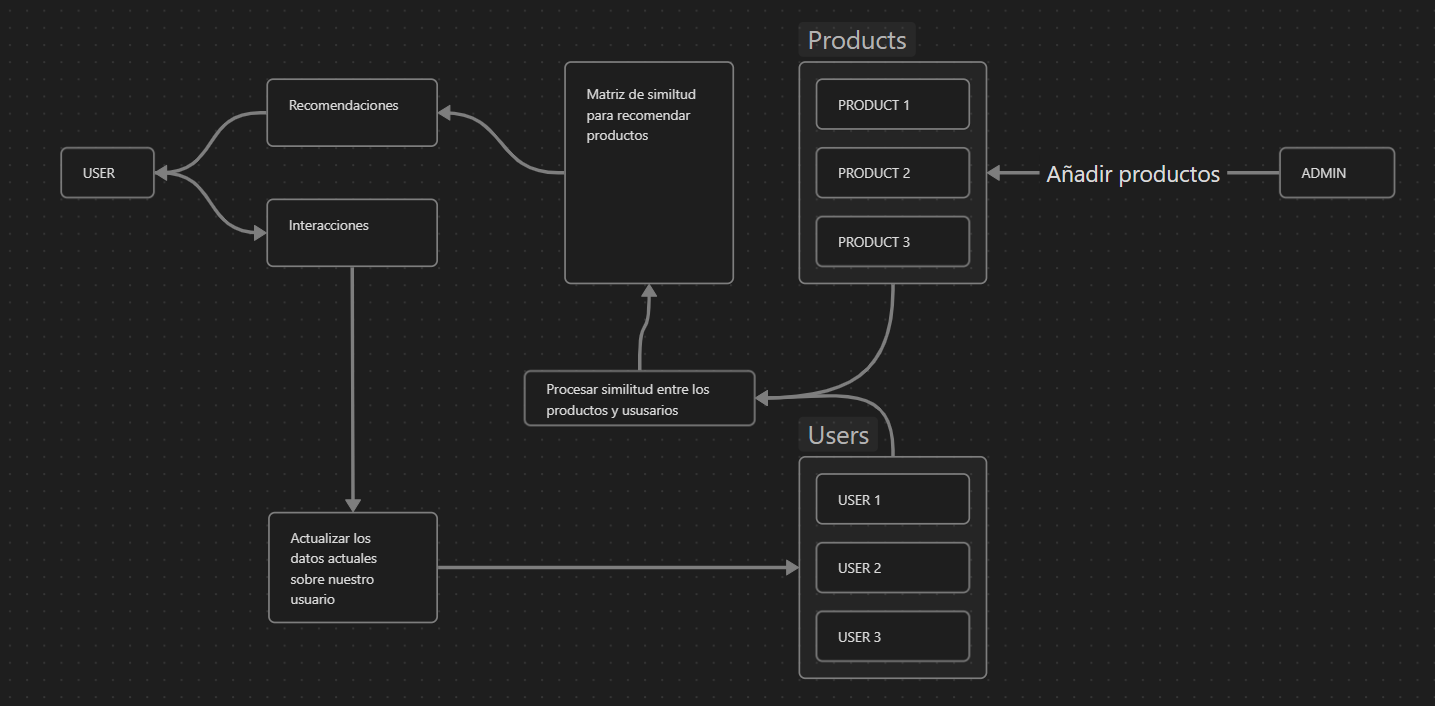
\includegraphics[width=0.8\textwidth]{workflow.png}
\caption{Flujo de trabajo del sistema de recomendación híbrido}
\label{fig:workflow}
\end{figure}

\end{document}
